% Fig. 2 -- fault-injection coverage matrix
% Included by paper/icc_main.tex via \input.
\begin{figure}[!t]
\centering
\resizebox{\columnwidth}{!}{%
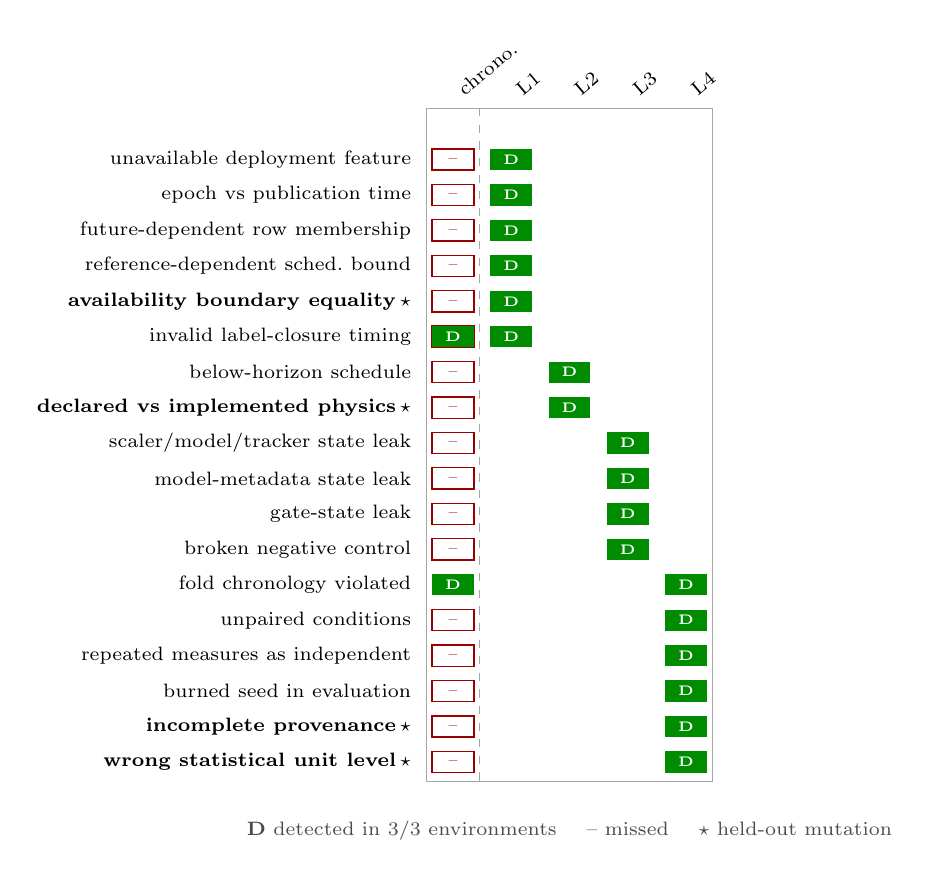
\begin{tikzpicture}[font=\scriptsize,x=7.4mm,y=4.5mm]
\def\hit#1#2{\fill[green!55!black] (#1-0.36,#2-0.30) rectangle (#1+0.36,#2+0.30);
  \node[white,font=\tiny\bfseries] at (#1,#2) {D};}
\def\mis#1#2{\draw[red!60!black,line width=0.5pt] (#1-0.36,#2-0.30) rectangle
  (#1+0.36,#2+0.30); \node[red!60!black,font=\tiny] at (#1,#2) {--};}
\foreach \c/\lab in {0/{chrono.}, 1/{L1}, 2/{L2}, 3/{L3}, 4/{L4}}
  \node[rotate=40,anchor=west,font=\scriptsize] at (\c,0.75) {\lab};
\foreach \r/\nm/\ho in {%
  1/{unavailable deployment feature}/0, 2/{epoch vs publication time}/0,
  3/{future-dependent row membership}/0, 4/{reference-dependent sched.\ bound}/0,
  5/{availability boundary equality}/1, 6/{invalid label-closure timing}/0,
  7/{below-horizon schedule}/0, 8/{declared vs implemented physics}/1,
  9/{scaler/model/tracker state leak}/0, 10/{model-metadata state leak}/0,
  11/{gate-state leak}/0, 12/{broken negative control}/0,
  13/{fold chronology violated}/0, 14/{unpaired conditions}/0,
  15/{repeated measures as independent}/0, 16/{burned seed in evaluation}/0,
  17/{incomplete provenance}/1, 18/{wrong statistical unit level}/1}
  {\node[anchor=east,font=\scriptsize] at (-0.55,-\r)
     {\ifnum\ho=1\textbf{\nm}\,$\star$\else\nm\fi};}
\foreach \r in {6,13} {\hit{0}{-\r}}
\foreach \r in {1,2,3,4,5,6} {\mis{0}{-\r}} \foreach \r in {7,8,9,10,11,12} {\mis{0}{-\r}}
\foreach \r in {14,15,16,17,18} {\mis{0}{-\r}}
\foreach \r in {6,13} {\fill[green!55!black] (0-0.36,-\r-0.30) rectangle (0+0.36,-\r+0.30);
  \node[white,font=\tiny\bfseries] at (0,-\r) {D};}
\foreach \r in {1,2,3,4,5} {\hit{1}{-\r}} \hit{1}{-6}
\foreach \r in {7,8} {\hit{2}{-\r}}
\foreach \r in {9,10,11,12} {\hit{3}{-\r}}
\foreach \r in {13,14,15,16,17,18} {\hit{4}{-\r}}
\draw[black!35] (-0.45,0.45) rectangle (4.45,-18.55);
\draw[black!35,dashed] (0.45,0.45) -- (0.45,-18.55);
\node[anchor=north,font=\scriptsize,text=black!70] at (2,-19.4)
  {\textbf{D} detected in 3/3 environments \quad -- missed \quad $\star$ held-out mutation};
\end{tikzpicture}}
\caption{Fault-injection coverage. Legacy chronological checks (left column, dashed
separator) detect $2/18$ classes---exactly the two that are ordering properties.
Contract layers L1--L4 detect $18/18$, in all three environments. The four held-out
mutations ($\star$) were defined before their rules were written; two had no
predecessor detector of any kind.}
\label{fig:coverage}
\end{figure}
